
\subsection{Implementation}
\label{sec:Implementation}

 \paragraph{Patch size and stride.} In order to capture each frequency band at the right level of detail, I do not upsample the images $L_l(X)$ and use a small $3 \times 3$ patch size. I experimented with larger patch sizes; however, this turned out to be counterproductive for the level of detail targeted, as details are blurred in larger patches. They also led to overfitting and were, in general, harder to optimise for. I used a stride of $1$, and hence patches overlap on the image plane. The overlapping patches are averaged while reconstructing the image.
 
 \begin{landscape}\centering
\vspace*{\fill}
\begin{figure}[htpb]
  \centering
  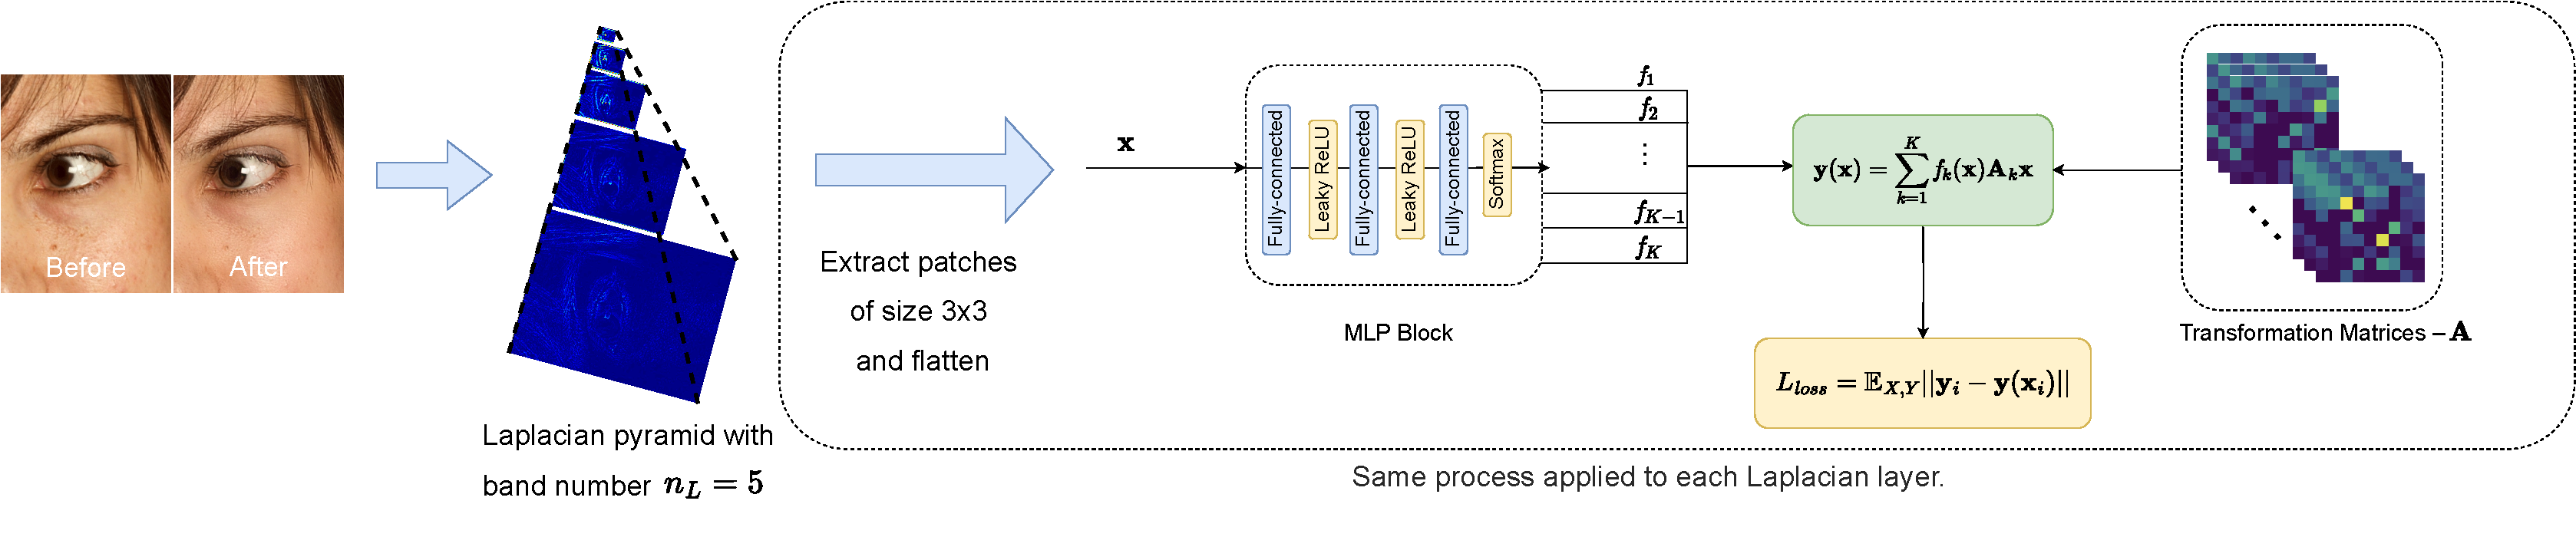
\includegraphics[width=1.5\textwidth]{Chapters/detail-retouching-figs/MainFig.pdf}
  \caption{The proposed technique learns a separate mapping per frequency band by decomposing images into five different bands with a Laplacian pyramid. At each Laplacian band $l$, a separate mapping is defined between flattened patches $\mathbf{x}_i$, $\mathbf{y}_i$ extracted from before-after bands $X_l$, $Y_l$. The field based method (MLP block) adapts transformations to input patches, providing local context-aware adjustments. The transformation matrices and MLP parameters are learned jointly from scratch for each Laplacian band of the before-after pair.}
 \label{fig:modelT}

\end{figure}
\vfill
\end{landscape}


\paragraph{Detail and colour modifications.} This work aims to capture intricate details present in highly detailed retouches and a wide range of image-processing operators. Based on the observation that various operators can edit materials in the image space using the luminance component~\cite{Boyadzhiev15Band}, I focus on learning changes in luminance while preserving the input chrominance channels.

\paragraph{Evaluation metrics.} To quantitatively compare the technique with state-of-the-art methods, I used Peak Signal-to-Noise Ratio (\gls{PSNR}) and Structural Similarity Index Measure (\gls{SSIM}) metrics. This is only possible if the before-and-after image pair was processed with a known, reproducible operator; see Section~\ref{sec:Comparisons} for details.

\paragraph{Training details.}\label{train_det} I train different mappings with the same structure, defined in Equation \ref{eq:weightedSum}, for each frequency band of the Laplacian pyramid. Each mapping consists of one \gls{MLP} block and $K$ number of transformation matrices, which are learned jointly for each frequency band from scratch for each before-and-after pair. The \gls{MLP} block employed in the experiments consists of three fully-connected layers and non-linearities applied after each layer. The output size of the last layer is the same as that of the number of transformation matrices.

To normalise the weights, I choose Softmax as the last activation function, while I apply Leaky \gls{ReLU} to the first two layers. Each transformation matrix is randomly initialised using a uniform distribution in the range of $[0, 1]$. All experiments use the Adam optimiser with a learning rate of $10^{-2}$, which exponentially decays with a decay rate of $0.96$. I use the $\mathcal{L}_{1}$ loss function in all experiments. Through backpropagation, both the \gls{MLP} parameters and the entries of the transformation matrices are jointly learned. The pseudocode for both the training and inference procedures is as follows:

\begin{algorithm}
\caption{One-shot Detail Retouching}
\SetKwFunction{FDetailRetouch}{Train}
\SetKwFunction{FPyramid}{LaplacianPyramid}
\SetKwFunction{FMLPBLOCK}{MLPBlock}
\SetKwFunction{FPatch}{ExtractPatch}
\SetKwFunction{Fprob}{Backpropagate}
\SetKwFunction{FDetailRetouchInf}{Inference}
\SetKwFunction{Fpatchmerge}{MergePatch}
\SetKwProg{Fn}{Function}{:}{}
\Fn{\FDetailRetouch{'before' image $X$, 'after' image $Y$}}{
	\Comment{Decompose images into its Laplacian bands.}\\
        $X_l \gets \FPyramid(X)$\;
        $Y_l \gets \FPyramid(Y)$\;
        
        \For{$l \gets 0$ \KwTo $n_l$}{
        \Comment{Extract patches from the bands..}\\
        $\mathbf{x}_i \gets \FPatch(X_l)$\;
        $\mathbf{y}_i \gets \FPatch(Y_l)$\;
        $f_k \gets \FMLPBLOCK(\mathbf{x}_i)$\;
        $\mathbf{y}(\mathbf{x}_i) \gets \sum^{K}_{k = 0} f_k(\mathbf{x}_i) \mathbf{A}_k \mathbf{x}_i$\;
        $\mathcal{L} \gets  = \mathbb{E}_{X, Y} || \mathbf{y}_i -   \mathbf{y} (\mathbf{x}_i) ||$\;  
        $(f_k, \mathbf{A}_k) \gets \Fprob(\mathcal{L})$}
        }
%\end{algorithm}

%\begin{algorithm}
%\caption{One-shot Detail Retouching}

\Fn{\FDetailRetouchInf{input image $I$, blending weights $f_k$, transformation matrices $\mathbf{A}_k$}}{

        $I_l \gets \FPyramid(I)$\;
        
        \For{$l \gets 0$ \KwTo $n_l$}{
        $\mathbf{i}_i \gets \FPatch(I_l)$\;
        \Comment{Transform input patches $\mathbf{i}_i$ with learned weights and matrices.}\\
        $\mathbf{o}_i \gets \sum^{K}_{k = 1} f_k(\mathbf{i}_i) \mathbf{A}_k \mathbf{i}_i$\;
        	\Comment{Place the patches on the output grid $O_l$.}\\
        $O_l \gets \Fpatchmerge(\mathbf{o}_i)$}
     
        \Comment{Sum all output bands with input residual.}\\
        $O = I_{n_l} + \sum_l O_l$\;
        \Return $O$}
        
\end{algorithm}

\newpage
\section{Results}
\label{sec:results}


\subsection{Ablation studies}\label{ablation}
The success of the learned mappings relies on two key components: patch-adaptive retouching and transformation blending. I therefore conduct experiments to illustrate their significance.

%Ifirst investigate the effect of the number of transformation matrices, $K$. 
% \paragraph*{Transformation Matrices.}
\paragraph{Transformation Matrices.} I compared transformation matrices of size $9 \times 9$ with scalar values. The method remained spatially varying, as I kept the \gls{MLP} unchanged and used $K=256$ scalar weights. I tested both methods on 100 images and computed the average \gls{PSNR} values. I observed that the technique using matrices outperformed the scalar values, even in simple algorithmic filters such as Gaussian and Unsharp Masking, achieving approximately 2 dB and 3 dB higher \gls{PSNR} values, respectively.

As the complexity of a retouching style depends on multiple factors, such as artists’ design choices, user preferences, and the artist toolbox, analysing such effects on retouching examples quantitatively is challenging. For simple algorithmic filters, such as Gaussian filters or unsharp masking, $K=1$ can sufficiently reproduce the filter. In contrast, more complex algorithms, such as bilateral filters, require more matrices to accurately capture the algorithmic edits (Figure \ref{fig:ablation_K}). Since retouching edits combine the effects of multiple operators and are highly non-linear, I found empirically that $K=256$ offers effective results for the retouching examples.


\begin{figure}[th] % "[t!]" placement specifier just for this example
    \centering
	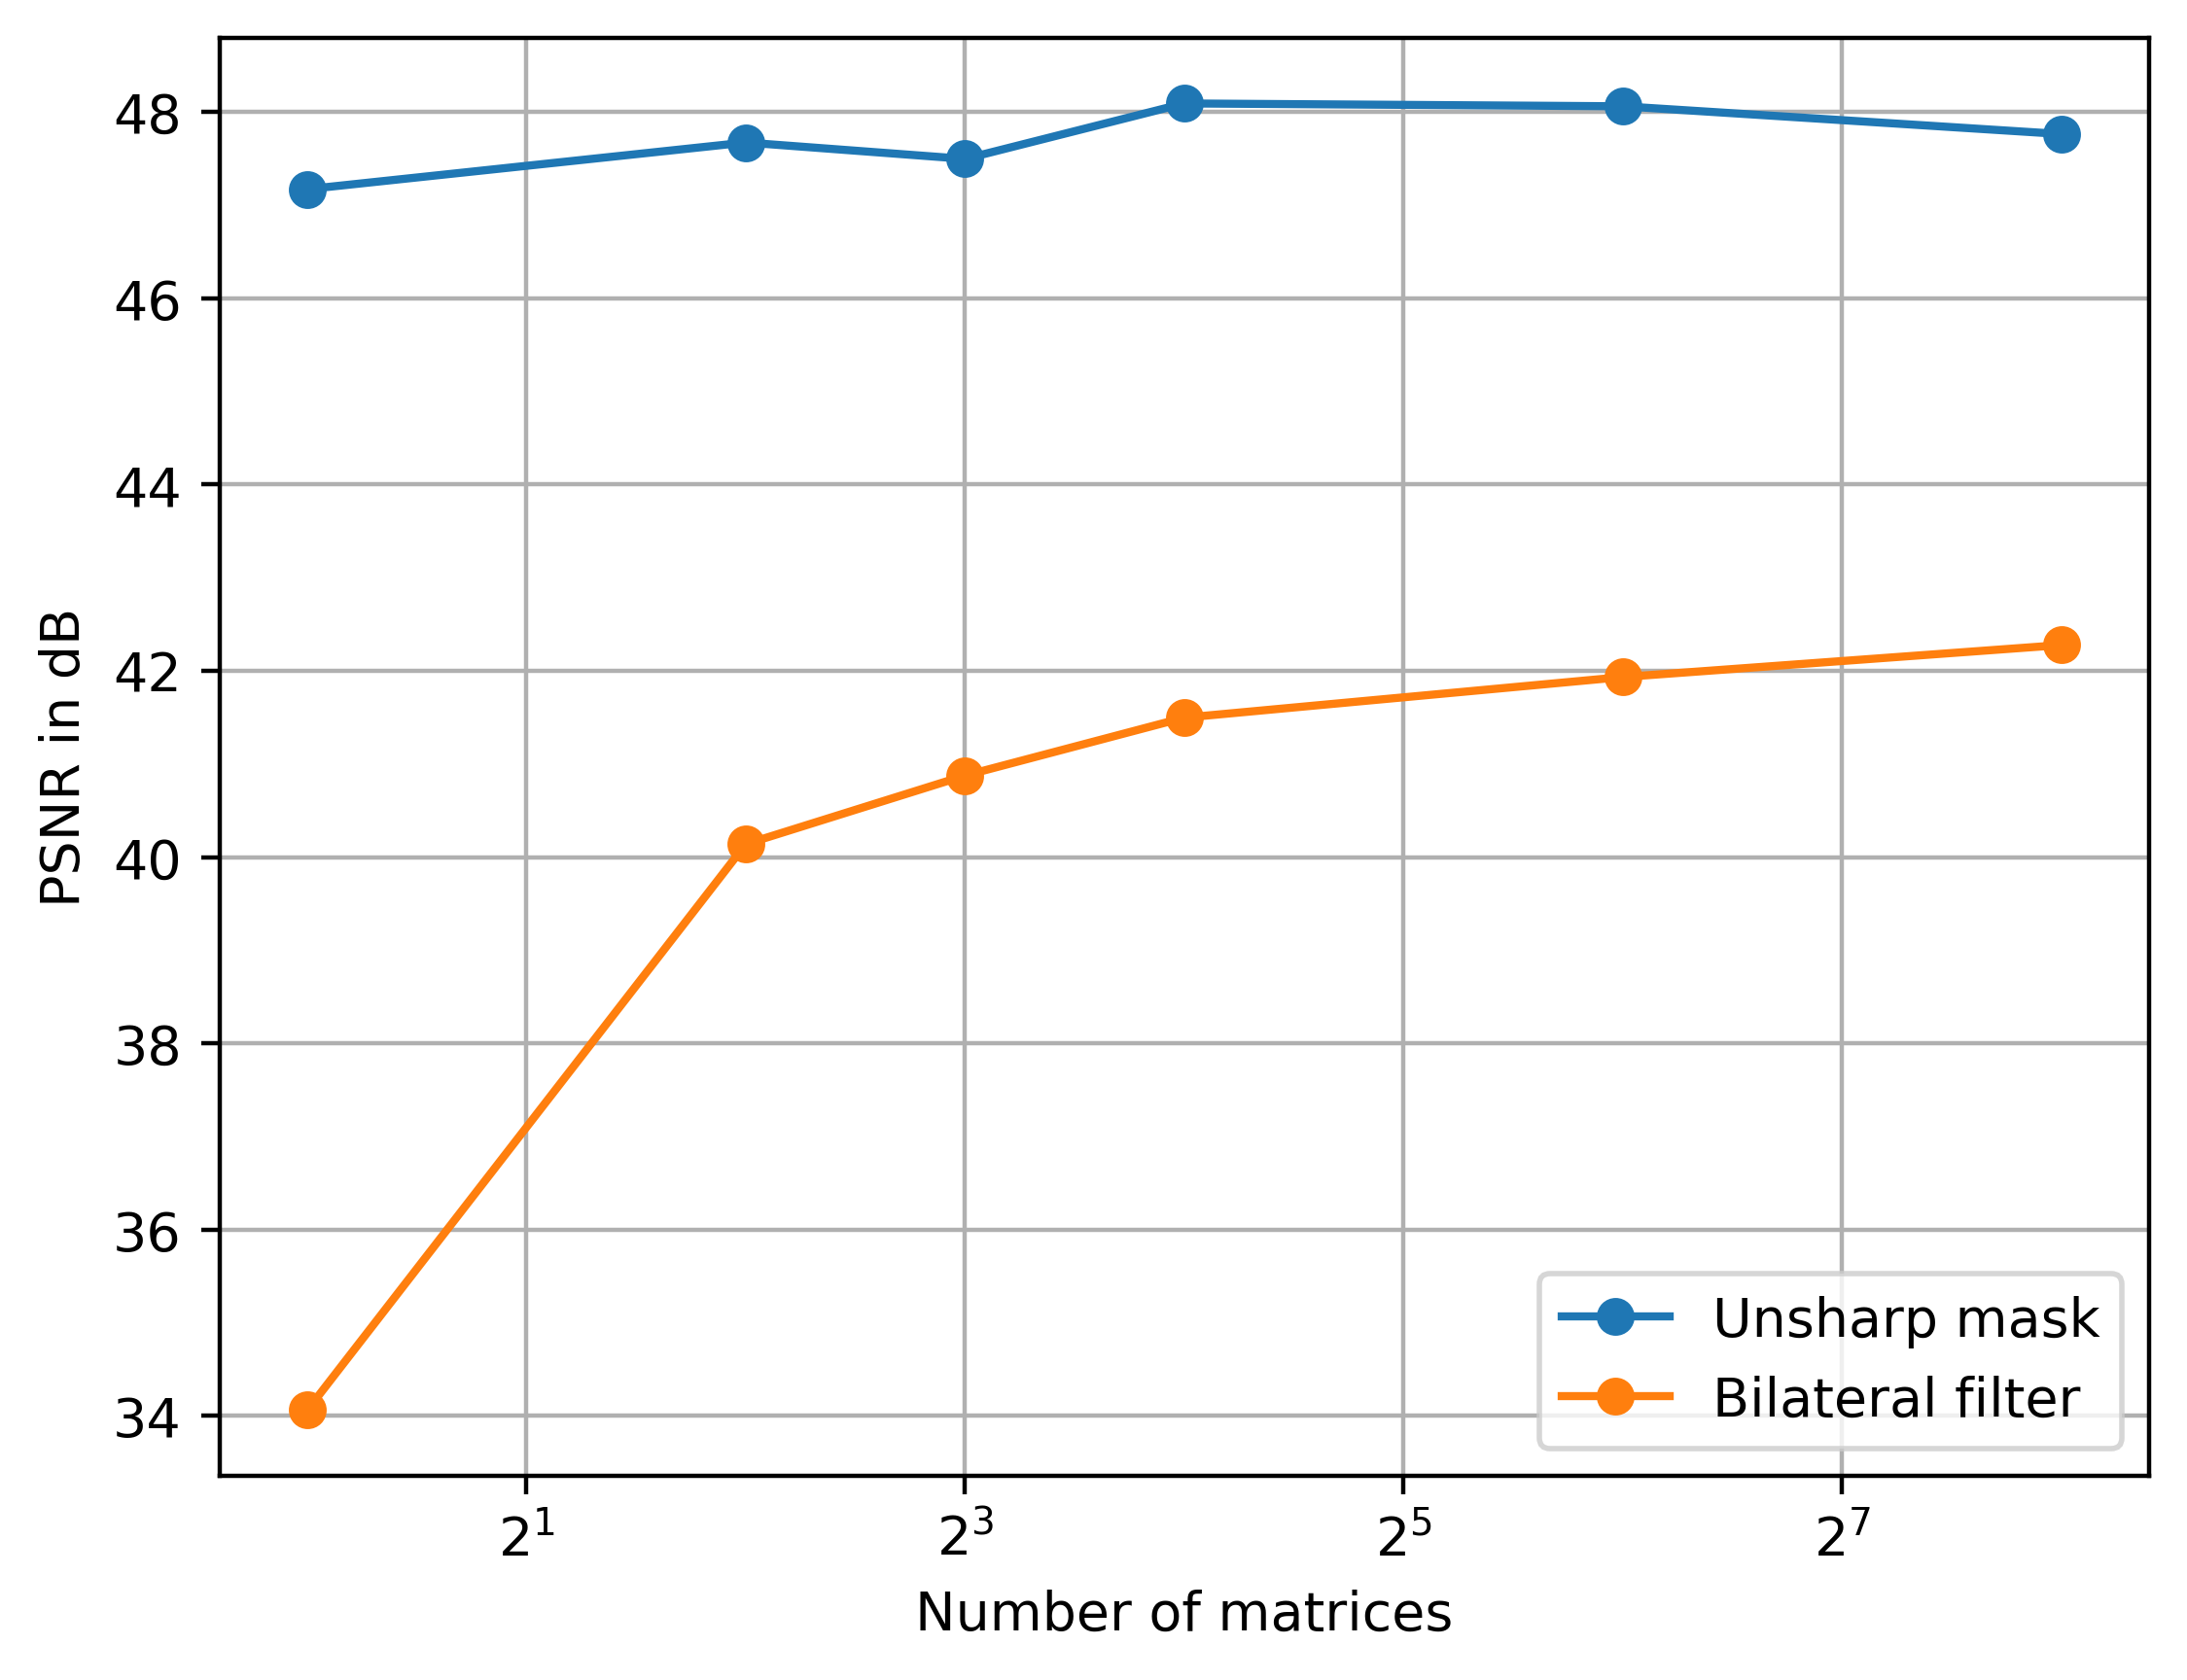
\includegraphics[width=0.6\columnwidth]{Chapters/detail-retouching-figs/ablation_matrices.png}

    \caption{The greater the complexity of the learned algorithm, the more transformation matrices the technique requires to accurately capture the effects on local regions. While $K=1$ can be sufficient for the model to capture unsharp masking, more matrices are required to accurately represent bilateral filtering.}

    \label{fig:ablation_K}
\end{figure}

\begin{figure}%[H]
\centering
\includegraphics[width=0.8\columnwidth]{Chapters/detail-retouching-figs/AblationStudy_K.pdf}
    \caption{An MLP regressor cannot effectively capture local edits, leading to inaccurate retouching results, such as blurring on the skin or around the eyes.}

\label{fig:ablation_MLP}
\end{figure}
% \paragraph*{Patch-adaptive Transformation Blending.}
\paragraph{Patch-adaptive Transformation Blending.} I also compared the patch-adaptive mapping with an \gls{MLP} regressor on the extracted patches. This directly learns the mapping from the decomposition of example before-after images instead of utilising blended transformations. The \gls{MLP} regressor follows a similar architecture to the \gls{MLP} block (Figure \ref{fig:modelT}), with the only difference being the last activation function. I used Leaky \gls{ReLU} here, since the Softmax function outputs pseudo-probabilities and is unsuitable for regression. Not explicitly addressing the spatially varying structure of the mapping limits the model’s expressiveness. This leads to blurry outcomes, as shown in Figure~\ref{fig:ablation_MLP}, because such a model cannot capture intricate detail edits, such as highlights around the eyes and hair or skin brightening. I also tried increasing the capacity of the \gls{MLP} regressor, but I did not observe significant improvement in performance.


\paragraph{Weights visualisation.} To study the effectiveness of the weights across an image, I randomly selected eight transformation matrices and reconstructed their corresponding weights for each Laplacian band. The reconstruction is performed similarly to how image patches are processed, with the weights placed in their respective locations. However, since each patch of size $3 \times 3$ has only one weight, I do not need to average over overlapping areas. I also cropped the last eight columns of the reconstructed weight images, as they contained zeros due to the size difference with the patches. Figure \ref{fig:weight-vis} displays the eight different reconstructed weights for each Laplacian band, obtained from the model trained with the example images shown in Figure~\ref{fig:DRteaser} (middle and right insets). The input to the model and the output retouched image are presented at the top. I observe the weights exhibit varying values across different regions in the bands. Note that the resolution of the bands has been increased for better visualisation; during training, each band’s resolution is maintained according to the Laplacian pyramid.


\begin{figure}%[H]
\centering
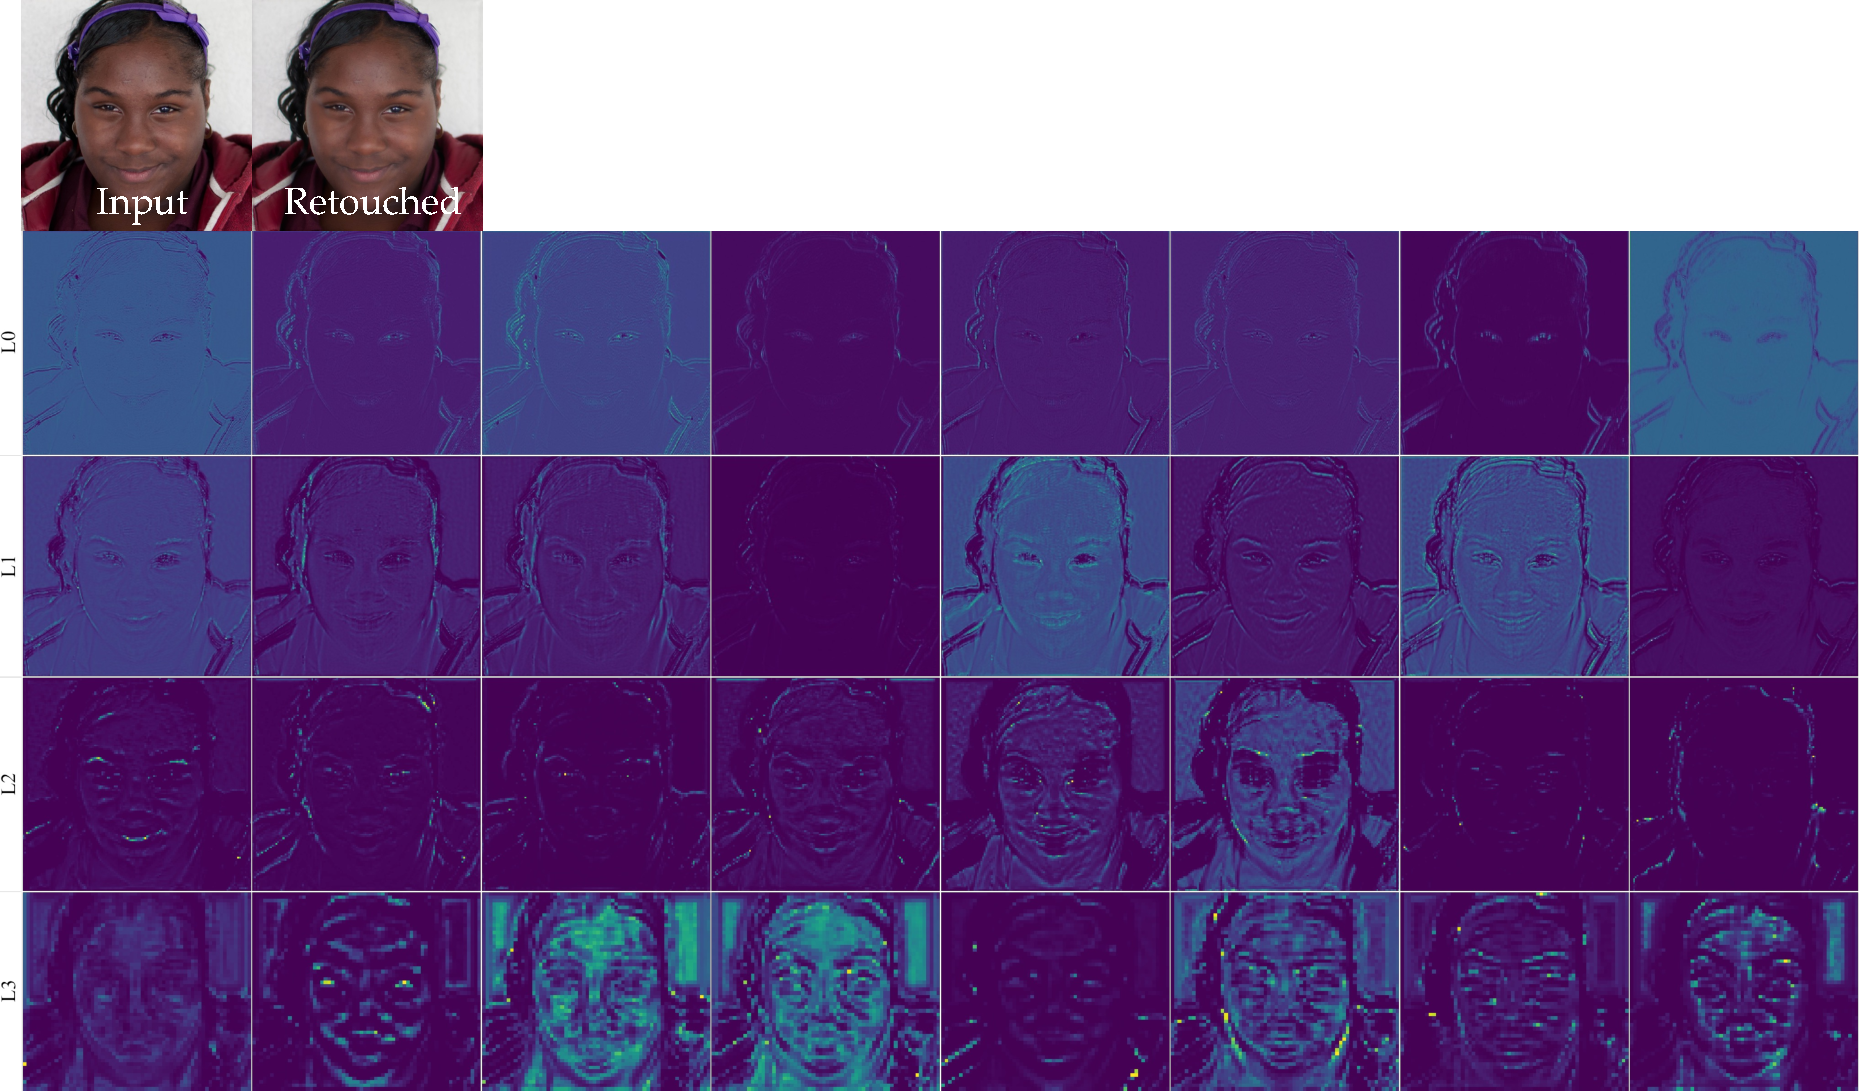
\includegraphics[width=\columnwidth]{Chapters/detail-retouching-figs/weight_visualise.pdf}
    \caption{Visualisation of the reconstructed patch-adaptive weights from the model trained with the example images in Figure~\ref{fig:DRteaser}. The input to the model is displayed at the top, and each row presents the weights corresponding to the indicated Laplacian band on the left.}

\label{fig:weight-vis}
\end{figure}

\subsection{Qualitative results}
 I tested the proposed technique on a diverse range of before-after pairs, including face images from the FFHQ dataset \cite{karras2019style}. I focus on human portraits and face retouching in the experiments, as they are arguably the most common and prioritised types of photos for retouching. I also illustrate that the technique provides visually pleasing results in different types of images, such as materials or rooms, and accurately captures image processing filters.
 
\begin{figure}[th] % "[t!]" placement specifier just for this example
    \centering
	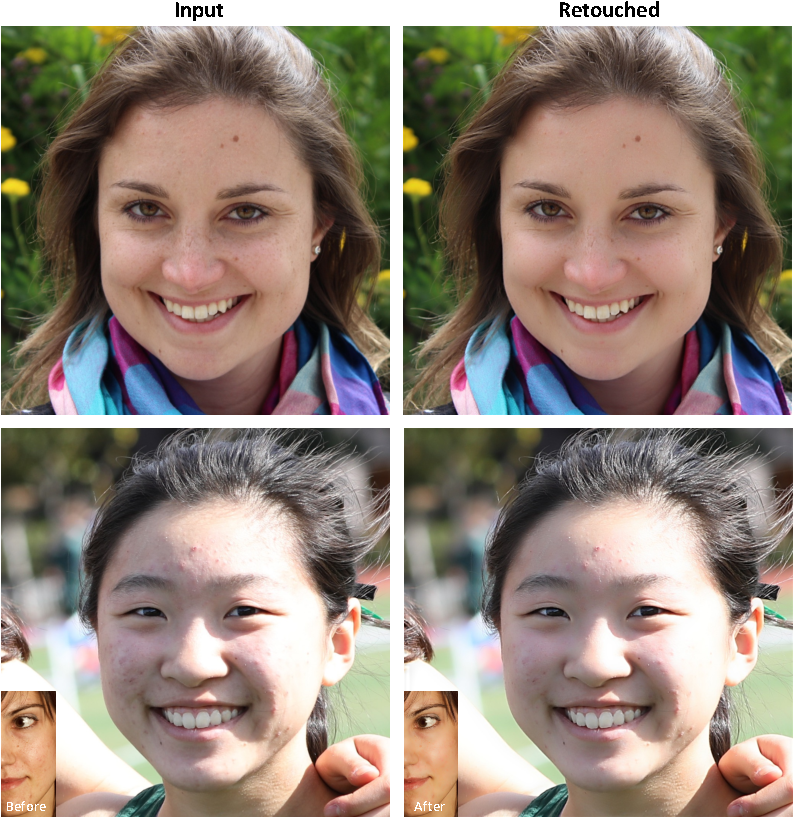
\includegraphics[width=0.8\columnwidth]{Chapters/detail-retouching-figs/res_diff_light_2_cvmp.pdf}
    \caption{\label{fig:newdataset_ex}The reproduced retouching style from the example pair (inset) improves skin texture without affecting fine details, such as the eyes and hair, resulting in a visually improved portrait. Moreover, the technique generalises well to faces under different lighting conditions and accurately reproduces the example retouching style.}
 
\end{figure}
% \paragraph*{Face retouching - skin and eye filters:}\label{faceretouching}
Human faces pose a particular challenge for the one-shot setting. However, the model can still capture highly nonlinear retouching edits and generalises well to different types of faces, view directions, and lighting conditions, as illustrated in Figures~\ref{fig:DRteaser}, ~\ref{fig:newdataset_ex}, and ~\ref{fig:retouchingstyles}.

\begin{figure}[th] % "[t!]" placement specifier just for this example
	\centering
	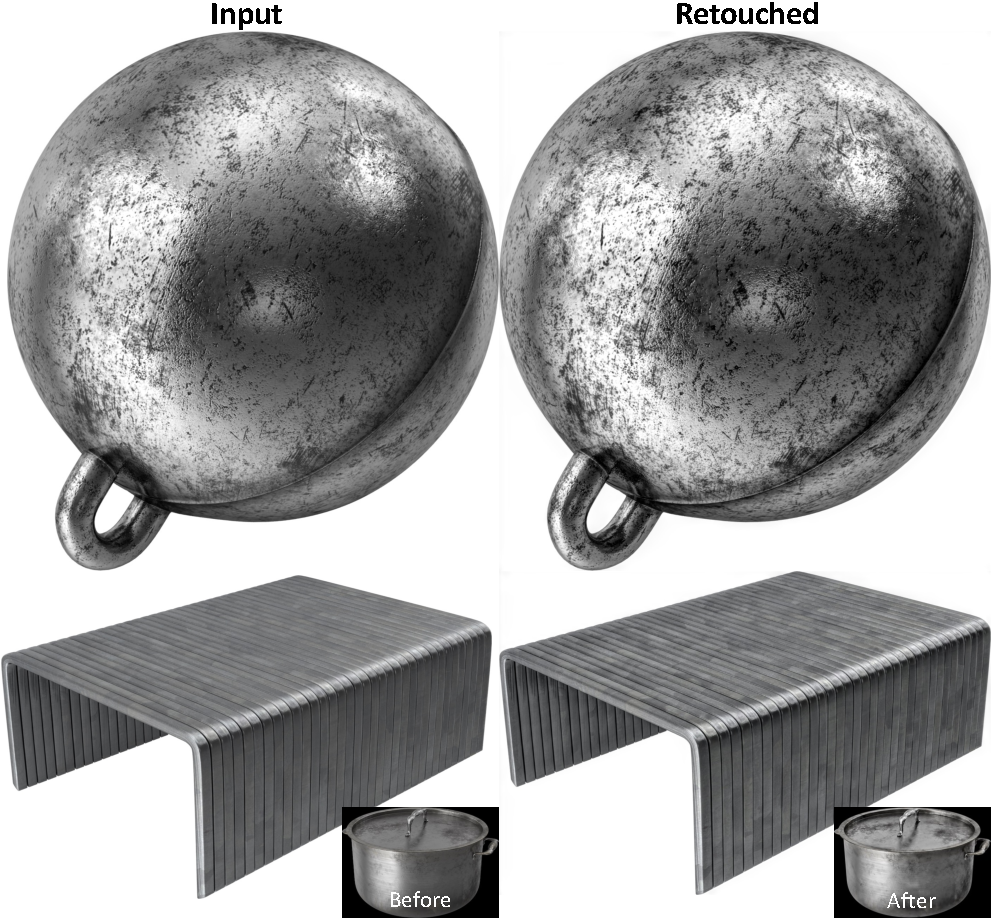
\includegraphics[width=0.8\columnwidth]{Chapters/detail-retouching-figs/MaterialResults.pdf}
    \caption{\label{fig:material_res}Material editing results on photos (left), and rendered images (right), based on the before-after pair (inset). The details, such as scratches or lines, are emphasised, and materials become shinier. Image courtesy of royalmix (top and bottom-inset), tsmdunn (bottom). (PixelSquid).}

\end{figure}

The example pairs in Figures~\ref{fig:DRteaser}, ~\ref{fig:newdataset_ex}  and ~\ref{fig:retouchingstyles} were produced by brushing onto the skin with artist-created brushes, eye sharpening (sharpening example in Figure~\ref{fig:DRteaser}), and further brightness/contrast adjustments. These brushes first decompose the skin into a detail and base layer, typically with frequency decomposition, alter the detail layer, and blend it with the base layer. They differ in how (1) they decompose the skin into the layers (i.e., which frequencies are in each layer), and (2) how they edit and blend each layer with different opacity values. This variation creates retouching nuances, as shown in~\ref{fig:retouchingstyles}. The framework can still accurately capture such slight differences in styles. 

\begin{figure}[th] % "[t!]" placement specifier just for this example
    \centering
	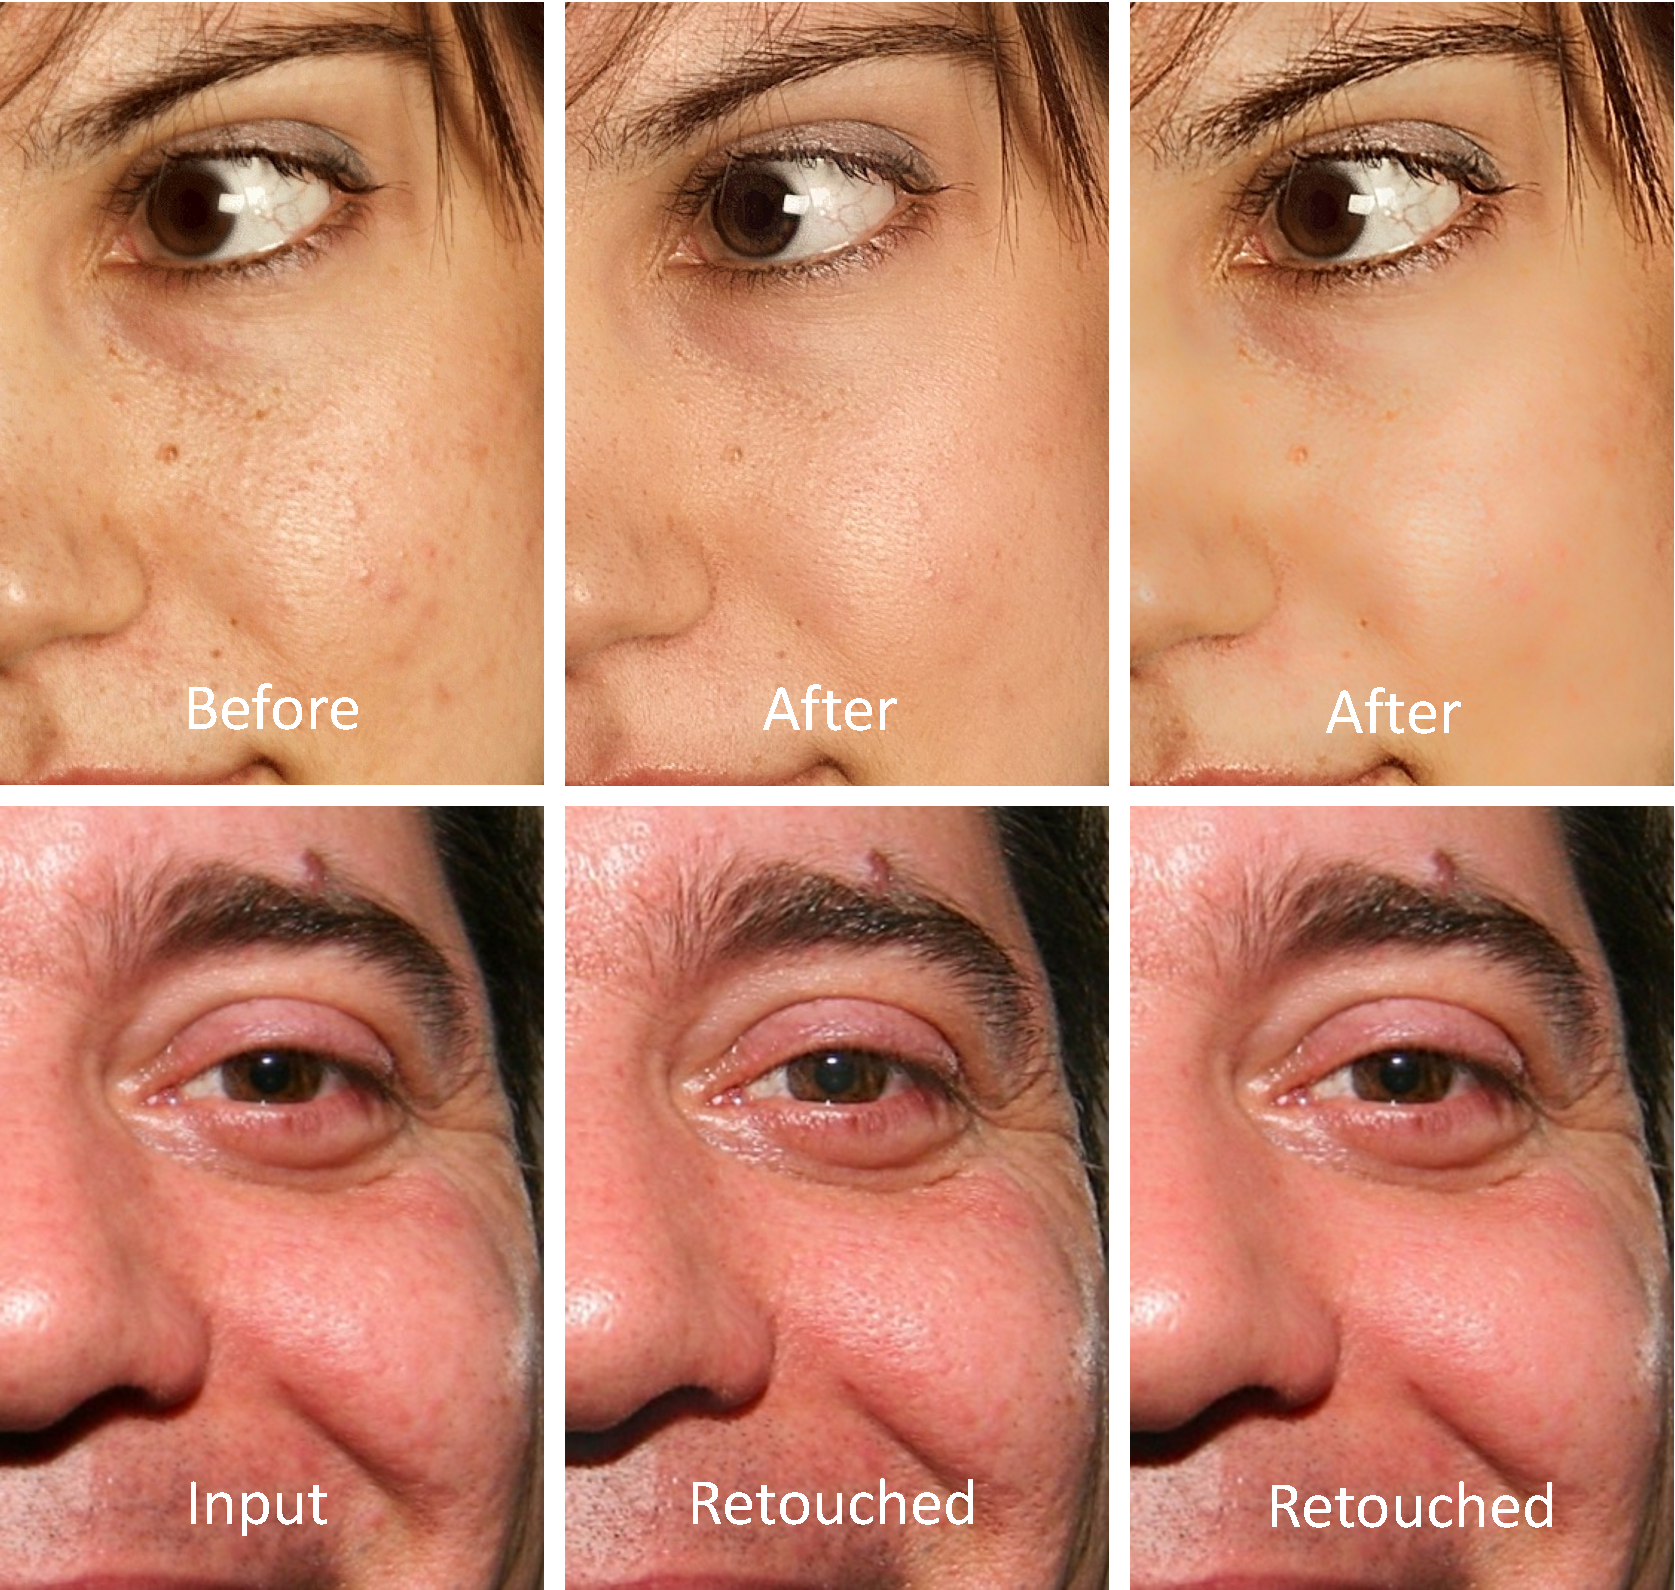
\includegraphics[width=\columnwidth]{Chapters/detail-retouching-figs/Nuances.pdf}
  % \hfill
    \caption{Our patch-adaptive technique can accurately capture the nuances between different
    retouching styles as given by the examples (top row).}
\label{fig:retouchingstyles}
\end{figure}


In all experiments, intricate details of the desired retouching, such as small-scale texture, eyes, facial hair, or material details, and global features, such as overall lighting and tone, are accurately reproduced. It is interesting to observe that the \emph{glamour} implied by, for example, the example retouching in Figure~\ref{fig:newdataset_ex} is transferred from the example pair very accurately without causing an artificial appearance. Zooming into the skin reveals that pores and wrinkles are minimised, and the blemishes and discolouring of the skin are eliminated. At the same time, depending on the retouching edit, details, such as eyes or material texture, are more highlighted or preserved, and delicate features, such as hair, are preserved well Figures ~\ref{fig:newdataset_ex}, ~\ref{fig:material_res} and ~\ref{fig:retouchingstyles}).

In summary, the proposed technique efficiently edits such intricate details, due to significantly distinct local statistics of the texture at multiple scales, without affecting overlying structures thanks to its spatially varying nature and frequency decomposition.

\subsection{Comparison with the state-of-the-art}
\label{sec:Comparisons}


Although there are various works related to automatic photo enhancement, to the best of our knowledge, none of them work with a single example pair for detail retouching. Therefore, I compare the results with closely related automatic image-to-image translation methods, namely U-Net \cite{ronneberger2015u}, ASAPNet generator \cite{shaham2021spatially}, and Deep edge-aware filters \cite{xu2015deep}.

I trained each network from scratch with a single \textit{before-after} pair. To train the U-Net architecture, I changed the activation function of its last layer to \gls{ReLU} and used the  $\mathcal{L}_{1}$ loss function with the Adam optimiser (same as ours). Similar to the proposed method, ASAPNet is also a spatially adaptive network. However, it is instead designed to hallucinate new details. Therefore, I trained their generator model in a similar fashion with  $\mathcal{L}_{1}$ loss, by removing the discriminator. After observing that bilinear downsampling in their model caused checkerboard artifacts, I removed this operator and learned an MLP per pixel, which made the model highly complex with too many parameters.


\begin{table*}[th]
\centering
\caption{Quantitative performance comparison for the reproduction of various image processing filters. Average \gls{PSNR} and \gls{SSIM} values are computed over 182 images of different types, including faces, landscapes, materials, and rooms. Additional qualitative results can be found in Appendix \ref{one-shot-add}. We highlight the \colorbox{blue!25}{best PSNR} and \colorbox{orange!25}{best SSIM} results.}

\resizebox{\textwidth}{!}{\begin{tabular}{l@{\hskip 0.2in}c@{\hskip 0.1in}c@{\hskip 0.1in}c@{\hskip 0.1in}@{\hskip 0.1in}c@{\hskip 0.1in}c@{\hskip 0.1in}c}
    % \begin{tabular}{@{}cccccc@{}}
    \toprule
     \multicolumn{5}{c}{{Comparison results (PSNR in dB / SSIM)}} \\ \cline{1-5}
     {Filter Type} & {ASAPNet Generator} & {Deep Edge-aware} & {UNet} & {Ours}\\
     \midrule
    Gaussian & \cellcolor{orange!25}{39.36 / 0.983} & 36.52 / 0.979 & 40.52 / 0.979 & \cellcolor{blue!25}{40.67 / 0.983} \\%\midrule
    %   \hline
     Unsharp Mask & 29.77 / 0.889 & 32.62 / \cellcolor{orange!25}{0.959} & 32.05 / 0.919 & \cellcolor{blue!25}{33.88 /
0.931}\\%\midrule
    %   \hline
     Bilateral Filter & 33.65 / 0.936 & 33.56 / 0.958 & 34.00 / 0.939 & \colorbox{blue!25}{38.16 / 0.965}\\%\midrule
    %   \hline
     Local Laplacian ($\alpha=2$, $\sigma =0.2$) & 30.85 / 0.913 & 30.69 / 0.943 & 31.53 / 0.925 & \cellcolor{blue!25}{33.50 / 0.950} \\%\midrule
    %   \hline
     Local Laplacian ($\alpha=0.5$, $\sigma =0.1$) & 31.98 / 0.909 & 31.62 / 0.931 & 33.08 / 0.929 & \cellcolor{blue!25}{35.72 / 0.940}

     \\\bottomrule
    %  \hline
    \end{tabular}}
\label{tablecomparison}
\end{table*}


% These results are included in Table 1 for the filter types indicated in rows. The training strategy for the state-of-the-art methods is summarised in Section \ref{sec:Comparisons}. Before-after pairs along with additional results can be found in the supplementary material. Image courtesy of Arnaud Rougetet (landscape) and virtualhorizonstudio (alarm clock). (CC-BY and PixelSquid)


To ensure a fair comparison with contemporary methods, I trained each network with the same example pair processed by four algorithmic filters: Gaussian, unsharp masking, bilateral, and local Laplacian filters (\gls{LLF}). As \gls{LLF}s can perform a wide range of edge-aware operations, I apply two different versions of the filter: one for smoothing ($\alpha=2, \sigma=0.2$) and one for enhancing details ($\alpha=0.5, \sigma=0.1$). Each network is trained from scratch with the same example pair resized to $256 \times 256$ for the corresponding filter.

%($\alpha=0.7, \sigma=0.4$)
%Itested the models with 100 face images, randomly sampled from MIT-Adobe FiveK \cite{Bychkovsky11Learning}, 
To prove the generalisability of the technique, I tested the models on different types of images, namely face images (100 images randomly sampled from MIT-Adobe FiveK \cite{Bychkovsky11Learning}), material images (22 images), room images (30), and landscape images (30). Each type was trained separately with its corresponding example pair. For instance, I trained an example pair of landscape images to test the model on landscape images. I evaluated the models using average \gls{PSNR} and \gls{SSIM} values. To generate the ground truth for the input images, I applied the same filter as was applied to the before example image to obtain the after image. I trained each model in the Y channel after converting RGB images to their YCbCr versions and evaluated the results for Y-channel images.

To obtain the U-Net results for each type of image, I ran an additional experiment in which I changed the number of trainable parameters by removing some layers and trained the network from scratch for unsharp masking and bilateral filtering. The number of chosen parameters was 0.1M (with a few convolutional layers), 1.8M, 10M, and 30M. For material images, I observed that 10M performed the best in terms of \gls{PSNR} and \gls{SSIM} values, whereas for other types of images, 30M performed best. I tested the trained models on the images of the corresponding types and computed average \gls{PSNR} values. Later, I chose the model with the best-performing parameters for each type of image for the quantitative comparison (Table \ref{tablecomparison}).

Overall, our method can outperform all architectures for each considered filter in terms of \gls{PSNR} values. U-Net shows the closest performance, but its network capacity is significantly higher than the proposed framework (0.16M). As the filter becomes more complex, the performance gap increases. For instance, other methods perform fairly well in simple algorithmic filters, such as Gaussian or unsharp masking. However, in spatially varying filters, namely the bilateral filter or \gls{LLF}s, the proposed method proves more generalisable thanks to its patch-adaptive structure.

Figures \ref{fig:QualitativeComp_BF}, \ref{fig:QualitativeComp_LLF_a2}, and \ref{fig:QualitativeComp_LLF_a05} further demonstrate that our technique can preserve and edit intricate details, such as text, texture, or leaves, more effectively without causing much distortion. Nonlinear bilateral filters and local Laplacian filters pose an additional challenge, especially in a one-shot setting. However, the proposed approach can still perform edge-aware filtering with higher accuracy than the baselines. Note that these examples are selected from the results obtained for the quantitative comparison (Table \ref{tablecomparison}), where only the luminance channels were used and the images were downsampled to $256 \times 256$.


\subsection{Limitations and future work}
\begin{figure}[th] % "[t!]" placement specifier just for this example
	\centering
	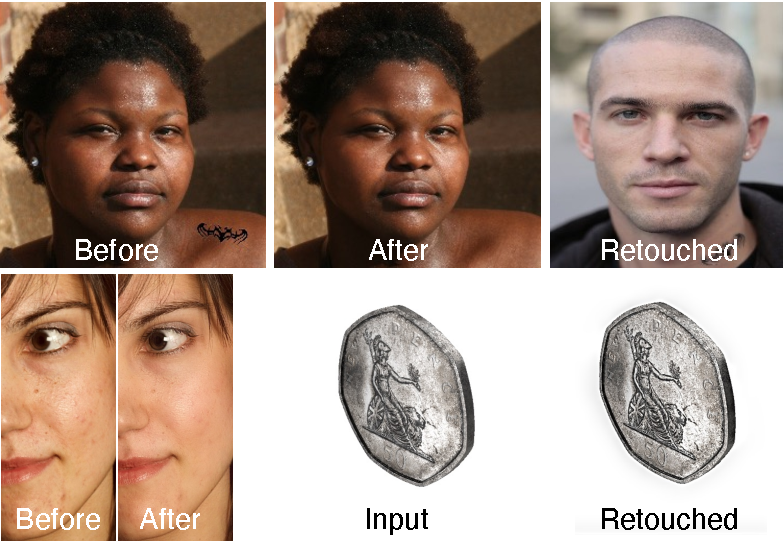
\includegraphics[width=0.8\columnwidth]{Chapters/detail-retouching-figs/Limitations.pdf}
    \caption{\label{fig:limitations} The proposed technique cannot accurately handle extreme non-repeating local effects, such as tattoos (top), and situations where the example and input images have very different semantics (bottom). Image courtesy of bgaj23 (coin). (PixelSquid).}

\end{figure}
A primary limitation of this work is its dependence on local patches at different scales, disregarding their spatial locations. Hence, the method is most useful when details are retouched based on the local and repeated characteristics of an image. Non-repeating spatially-dependent effects, such as tattoos or portrait stylisations with spatially varying lighting~\cite{Shih14Style}, cannot be handled by the current technique; see Figure \ref{fig:limitations}.

Since the method relies on a single example image pair, transferring filters applied to arbitrary images~\cite{Yan14Automatic} is beyond the scope of this work. The example and input images need to have similar semantics for predictable transfer. Extending the technique to include more than one pair of example images will require consistently retouched details across all those examples. Lastly, the example before and after images must be perfectly aligned. This requirement could be mitigated by incorporating an ICP~\cite{Besl92AMethod}-like approach into the optimisation process in Section~\ref{sec:Methodology}. 

Although the primary focus of this paper is on learning artist-driven subjective retouching edits, the proposed technique is generalisable. It can be extended to transfer arbitrary image transformations, particularly where details are modified. Therefore, I plan to further investigate the technique as a general transfer method for image-to-image translation. The patch-adaptive nature of the mappings makes them amenable to analysis.

\begin{figure*}%[th]%[tph]{
  \centering
      
\includegraphics[width=.82\linewidth]{Chapters/detail-retouching-figs/One-shot-labels.pdf}

  \includegraphics[width=\linewidth]{Chapters/detail-retouching-figs/Qualitative_zoomed_BF.pdf}
    \caption{Qualitative comparison with baseline approaches on bilateral filtering. The bilateral filter is a non-linear filter designed for smoothing surfaces while preserving edges. Results demonstrate that our proposed technique captures the bilateral filtering effect more effectively, reducing surface roughness while maintaining essential details.} 

   \label{fig:QualitativeComp_BF}%
\end{figure*}

 %   These results are included in Table 1 for the filter types indicated in rows. The training strategy for the state-of-the-art methods is summarised in Section \ref{sec:Comparisons}. Before-after pairs along with additional results can be found in the supplementary material. Image courtesy of Arnaud Rougetet (landscape) and virtualhorizonstudio (alarm clock). (CC-BY and PixelSquid).

\begin{figure*}%[th]%[tph]{
  \centering
      
\includegraphics[width=.82\linewidth]{Chapters/detail-retouching-figs/One-shot-labels.pdf}
  \includegraphics[width=\linewidth]{Chapters/detail-retouching-figs/Qualitative_zoomed_LLF_a2_s02.pdf}
    \caption{Qualitative comparison with baseline approaches on Local Laplacian filter (LLF) ($\alpha=2, \sigma=0.2$). LLF is another edge-aware non-linear filter designed for multiple tasks, including edge-preserving smoothing, detail enhancement, tone mapping, and inverse tone mapping. In these examples, the parameters are chosen to produce an edge-preserving smoothing effect, similar to bilateral filtering. Results show that our method offers smoother textures.} 

   \label{fig:QualitativeComp_LLF_a2}%
\end{figure*}

%These results are included in Table 1 for the filter types indicated in rows. The training strategy for the state-of-the-art methods is summarised in Section \ref{sec:Comparisons}. Before-after pairs along with additional results can be found in the supplementary material. Image courtesy of Arnaud Rougetet (landscape) and virtualhorizonstudio (alarm clock). (CC-BY and PixelSquid).

\begin{figure*}%[th]%[tph]{
  \centering
    
\includegraphics[width=.82\linewidth]{Chapters/detail-retouching-figs/One-shot-labels.pdf}
  \includegraphics[width=\linewidth]{Chapters/detail-retouching-figs/Qualitative_zoomed_LLF_a05_s01.pdf}
    \caption{Qualitative comparison with baseline approaches on Local Laplacian filter (LLF) ($\alpha=0.5, \sigma=0.1$). Here, the parameters are chosen to enhance the details. Our results highlight edges, such as the transition between the cloud and the sky, the numbers on the clock, and the texture of the bed sheet.} 

   \label{fig:QualitativeComp_LLF_a05}%
\end{figure*}